% Research Issues and Methodology in Language (SHSM 6020)
% Session 2
% Thomas Klee
% 2019-02-25

\documentclass[10pt, a4paper]{article}   	% use "amsart" instead of "article" for AMSLaTeX format
\usepackage{geometry}                		% See geometry.pdf to learn the layout options. There are lots. Uncomment to narrow margins
%\geometry{letterpaper}                   		% ... or a4paper or a5paper or ... 
%\geometry{landscape}                		% Activate for for rotated page geometry
%\usepackage[parfill]{parskip}    		% Activate to begin paragraphs with an empty line rather than an indent
\usepackage{graphicx}				% Use pdf, png, jpg, or eps§ with pdflatex; use eps in DVI mode
								% TeX will automatically convert eps --> pdf in pdflatex		
\usepackage{amssymb}

\usepackage[colorlinks = true, linkcolor = blue, urlcolor = blue, citecolor = black]{hyperref} 
\newcommand{\sourcefile}{\url}

\usepackage{scrextend} 
\addtokomafont{labelinglabel}{\sffamily}

\title{Instructions for Downloading and Installing R and RStudio}
\author{Thomas Klee}
\date{2019-02-25}							% Activate to display a given date or no date

\begin{document}
\maketitle

When we meet in class on Saturday, I'll introduce you to a computer program called R so that you can think about whether it would be useful in your own research. I'll introduce you to some basic operations in R and demonstrate how to analyse data for a meta-analysis. In preparation for this, please download and install two computer programs on your laptop. Please bring your laptop to class. 

\section*{First, a little background\dots}

R is an open-source statistical software package. It's not a point-and-click program like other stats programs you may have used (e.g. SPSS) and because of that, it has many advantages. One is that, unlike SPSS, you will still be able to use R after you graduate without having to pay an annual license fee.

\section*{Now, the instructions\dots}

Download and install R and RStudio on your computer before class. Both are free. R is the statistics package and RStudio is a program that makes R much easier to use, in that it integrates R with many other useful resources and keeps your R commands and statistics output nicely organised.

\subsection*{R}
First, download and install R. 

\begin{enumerate}
	\item Go to \url{https://cloud.r-project.org} 
	\item Click on the version for your computer's operating system
		\begin{enumerate}
			\item For Mac OS X, get the latest release: \texttt{R-3.5.2.pkg} as of document date 
			\item For Windows, click on \texttt{install R for the first time}, and then \texttt{Download R 3.5.2 for Windows}. R comes in 32-bit and 64-bit versions for Windows. More about this can be found on the same web page by clicking on \texttt{Should I run 32-bit or 64-bit R?} If you don't know which version of Windows your laptop runs, {\href{https://support.microsoft.com/en-hk/help/827218/how-to-determine-whether-a-computer-is-running-a-32-bit-version-or-64}{click here}}. 
		\end{enumerate}
	\item Double-click the program icon to install. Let it install to your computer's default location.
\end{enumerate}

\subsection*{RStudio}
Second, download and install RStudio. The current version is 1.1.463 as of document date.

\begin{enumerate}
	\item Go to \url{https://www.rstudio.com}
	\item Click the \texttt{Download} link under the \textbf{RStudio} graphic on the left.
	\item Click the \texttt{Download} link in the \textbf{RStudio Desktop} column.
	\item Click on the installer for your operating system (e.g. Windows or Mac OS X). No need to download any Zip/Tarballs on that page.
	\item When the program has downloaded onto your desktop, double-click the program icon to install. Let it install to your computer's default location. If it's not on your desktop, check your Downloads folder and double-click on the file there.
	\item Move the RStudio program to your Mac's dock or your PC's desktop to access the program easier. When you click on the RStudio icon, your screen should look something like the image below. If R installed properly, you should see some lines of text in the bottom left panel.
	\item R is accessed via RStudio, so you should never have to click on the R icon itself unless you want to upgrade R to the next version.
\end{enumerate}

\begin{figure}[h]
\centering
	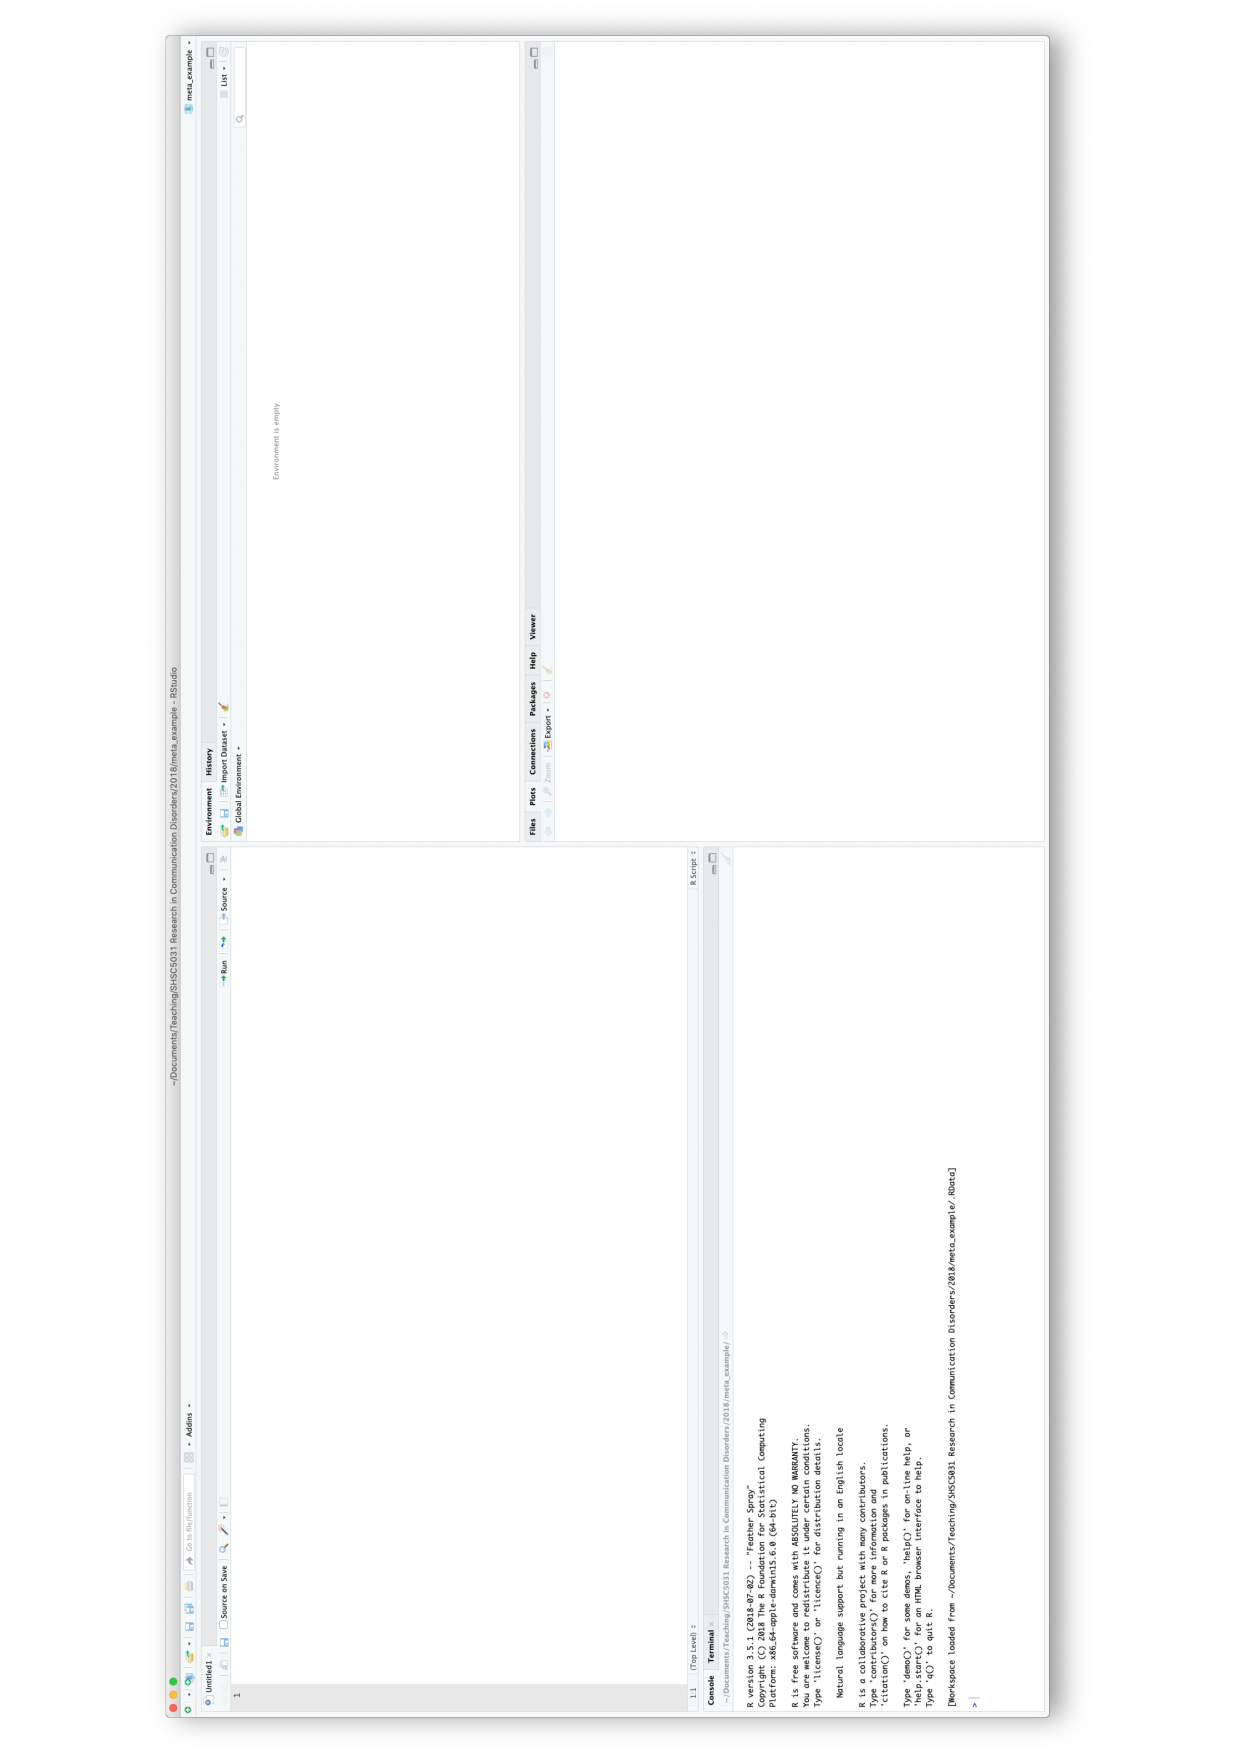
\includegraphics[angle = 270, width = \textwidth]{images/rstudio_screenshot.pdf}
\end{figure}

\section*{What's next?}
Once you've installed both programs, you'll be ready to begin using R. You don't need to do anything before class. At that time, I'll do a basic introduction to RStudio, R and R packages. I'll also show you what a meta-analysis using R looks like and we'll go through the steps of doing a meta-analysis with R. It's important that you ask questions when things aren't clear rather than holding back, so interaction in class is encouraged! 

\begin{labeling}{Warning}
	\item [Warning] Don't try to learn R when you have a deadline looming. R takes time to learn and it's best to do it in small chunks. It is a kind of programming language, with its own vocabulary and syntax, and you'll be learning to write code, so patience is required. Fortunately, there are many wonderful resources on the web for getting help and I can point you to what some of them are. 
	
	R has a huge and supportive network of users out there---and the question you have is likely to have already been asked and answered by someone else. One of the most challenging (and interesting) things about R is that there is usually more than one way to do something. This can be frustrating in the early stages of learning R but you'll come to appreciate how flexible the program is. 
\end{labeling}

\end{document}  